

\actTitle{Worksheet 4.3}



\noindent \textbf{Instructions:}  Work together in groups of  3 or 4 to complete the following problems.\\

Student goals:
\begin{itemize}
\item Determine values of trigonometric functions given right triangles.
\item Use the Pythagorean identity to determine the value of one
  trigonometric function in terms of another.
\item Determine the values of trigonometric functions using multiple
  right triangles.
\item Translate a written description of a problem into a
  trigonometric formulation
\end{itemize}


\begin{enumerate}

\item Find the exact values of the six trigonometric functions of $\theta$ and $\alpha$
\begin{enumerate}
\item Use the following triangle.\\
\trigTriangle{$\theta$}{$\alpha$}{8}{10}{~}
\vfill

\item Use the following triangle.\\
\trigTriangle{$\theta$}{$\alpha$}{15}{~}{8}
\vfill
\end{enumerate}

\clearpage 

\item Use the isosceles right triangle and the 30/60/90 triangle to complete the table.

\begin{table}[h]
\begin{tabular}{|l|m{.12\textwidth}|m{.12\textwidth}|m{.12\textwidth}|m{.12\textwidth}|m{.12\textwidth}|m{.12\textwidth}|}
\hline
\textbf{$\theta$}        & \textbf{$\sin(\theta)$} & \textbf{$\cos(\theta)$} & \textbf{$\tan(\theta)$} & \textbf{$\csc(\theta)$} & \textbf{$\sec(\theta)$} & \textbf{$\cot(\theta)$} \\ \hline
30$^\circ=\frac{\pi}{6}$ &                         &                         &                         &                         &                         &                         \\  [2em] \hline
45$^\circ=\frac{\pi}{4}$ &                         &                         &                         &                         &                         &                         \\  [2em] \hline
60$^\circ=\frac{\pi}{3}$ &                         &                         &                         &                         &                         &                         \\  [2em] \hline
\end{tabular}
\end{table}

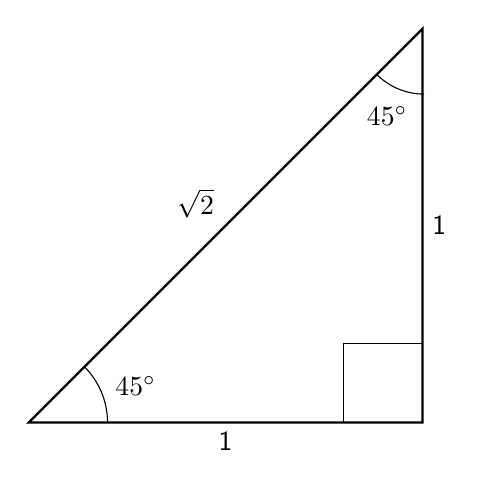
\begin{tikzpicture}[y=5cm, x=5cm,font=\sffamily]
  \draw[thick,black] (0,0) -- (1,0) -- (1,1) -- cycle;
  \draw[very thin,black] (0.8,0.0) -- (0.8,0.2) -- (1,0.2);
  \draw[thin,black] (0.2,0) arc (0:45:0.2);
  \node[black,anchor=north] at (0.5,0) {1};
  \node[black,anchor=west] at (1,0.5) {1};
  \node[black,anchor=south east] at (45:0.7) {$\sqrt{2}$};
  \node[black,anchor=south west] at (12.5:0.2) {$45^\circ$};
  \draw[thin,black] (45:1.25) arc (225:270:0.17);
  \node[black,anchor=west,xshift={8pt}] at (45:1.1) {$45^\circ$};
\end{tikzpicture}

\begin{tikzpicture}[y=5cm, x=5cm,font=\sffamily]
  \draw[thick,black] (0,0) -- (1,0) -- (60:2) -- cycle;
  \draw[thick,black,dashed] (1,0) -- (2,0) -- (60:2);
  \draw[very thin,black] (0.8,0.0) -- (0.8,0.2) -- (1,0.2);
  \draw[thin,black] (0.2,0) arc (0:60:0.2);
  \node[black,anchor=north] at (0.5,0) {1};
  \node[black,anchor=north] at (1.5,0) {1};
  \node[black,anchor=west] at (1,0.8) {$h$};
  \node[black,anchor=south east] at (60:1) {$2$};
  \node[black,anchor=south west] at (30:1.75) {$2$};
  \node[black,anchor=south west] at (12.5:0.2) {$60^\circ$};
  \draw[thin,black] (60:1.8) arc (240:270:0.2);
  \node[black,anchor=west] at (60:1.65) {$30^\circ$};
  \draw[thin,black] (1.8,0) arc (180:120:0.2) node[pos=0.5,anchor=south east] {$60^\circ$};
  \draw[thin,black] (1,1.535) arc (270:300:0.2) node[pos=0.,anchor=north west,yshift=-7] {$30^\circ$};
\end{tikzpicture}

\vfill

%\item
%\begin{enumerate}
%\item Evaluate $\sin(60^\circ)$.\\[0.2in]
%\item Evaluate $\sin(30^\circ)+\sin(30^\circ)$.\\[0.2in]
%\item Are the values in parts $(a)$ and $(b)$ the same?
%\end{enumerate}

\clearpage




\item For each problem below determine the values of the missing
  quantities. All angles are in radians, and your answers for angles
  should be in radians. (The triangles are not drawn to scale.)
\begin{enumerate}

\item ~ \\
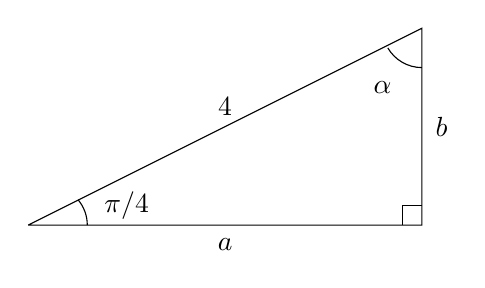
\begin{tikzpicture}[scale=2.5]
  \draw (0,0) -- (2,0) -- (2,1) -- (0,0);
  \draw (1.9,0) -- (1.9,0.1) -- (2,0.1);
  \draw (0.3,0) arc(0:40:0.2);
  \draw (0.5,0.1) node { $\pi/4$ };
  \draw (1.8,0.7) node { $\alpha$ };
  \draw (1,-0.1) node { $a$ };
  \draw (1,0.6) node { 4 };
  \draw (2,0.8) arc(270:210:0.2);
  \draw (2.1,0.5) node { $b$ };
\end{tikzpicture}
	
\framebox[0.3\textwidth][l]{
  \begin{tabular}{lc}
    $a$ & $=$ \\ [15pt]
    $b$ & $=$ \\ [15pt]
    $\alpha$ & $=$ \\
  \end{tabular}
}

\vfill

\item ~ \\
  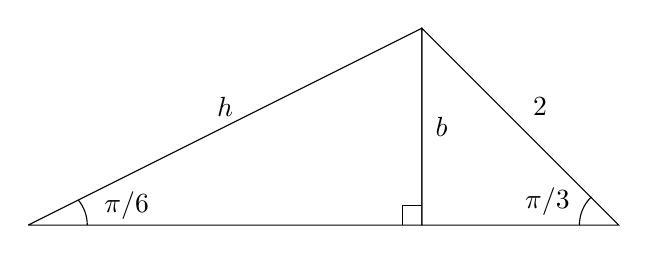
\begin{tikzpicture}[scale=2.5]
    \draw (0,0) -- (2,0) -- (2,1) -- (0,0);
    \draw (1.9,0) -- (1.9,0.1) -- (2,0.1);
    \draw (0.3,0) arc(0:40:0.2);
    \draw (0.5,0.1) node { $\pi/6$ };
    \draw (1,0.6) node { $h$ };
    \draw (2.1,0.5) node { $b$ };
    \draw (2,0) -- (3,0) -- (2,1) -- (2,0);
    \draw (2.8,0) arc(180:134:0.2);
    \draw (2.8,0) node[anchor=south east] { $\pi/3$ };
    \draw (2.6,0.6) node { $2$ };
  \end{tikzpicture}

	
  \framebox[0.3\textwidth][l]{
    \begin{tabular}{lc}
      $h$ & $=$ \\ [15pt]
      $b$ & $=$ \\ [15pt]
    \end{tabular}
  }
  
  \vfill

\end{enumerate}
\clearpage

\item A 30 ft boat ramp makes a $7^\circ$ angle with the water.  What
  is the height of the ramp above the water at the ramp's highest
  point?  Round to the nearest tenth of a foot.

  \vfill


\item At a tree farm, palm trees are harvested once they reach a
  height of 20 feet.  Suppose a farm worker determine's that the
  distance along the ground from her position to the base of a palm
  tree is 22 feet.  She then uses an instrument called a clinometer
  held at her eye level of 6 feet to measure the angle of elevation
  tot he top of the tree as $30.2^\circ$.  Is the tree tall enough to
  harvest?

  \vfill

  \clearpage

\item Robert Stroud is standing on top of a building, and he sees a
  pigeon on the ground away from the building. Robert’s angle of
  depression is $8.5^\circ$ as he stares at the bird. The bird hops
  15m directly away from the building, and the new angle of depression
  is $7.0^\circ$ .  What is the height of the building?


  \vfill

\end{enumerate}

\hwTitle{Section 4.3}

\begin{enumerate}
\item For each diagram below determine the values of the requested
  quantities.  All angles are in radians. (Figures are not drawn to
  scale.)

  \begin{enumerate}
    \item ~ \\

    \begin{minipage}[h]{0.4\linewidth}
      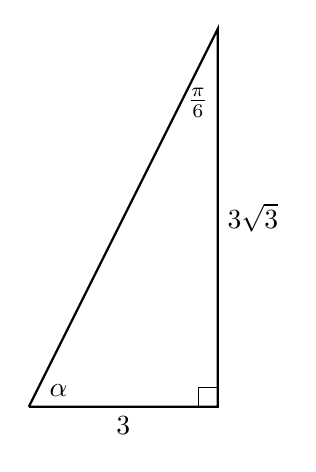
\begin{tikzpicture}[y=1.2cm, x=1.2cm,font=\sffamily]
        %% Draw the base, upright and hypotenuse
        \draw[thick] (0,0) -- (2,0) -- (2,4) -- (0,0); 
        \draw[thin] (0.9*2,0) -- (0.9*2,0.1*2) -- (2,0.1*2);
        \node[anchor=north] at (2/2,0) {$3$}; 
        \node[anchor=west] at (2,4/2) {$3\sqrt{3}$}; 
        %\node[anchor=south east] at (2/2,4/2) {$$};
        \node[anchor=south west,xshift=4] at (0,0) {$\alpha$};
        \node[anchor=north east,yshift=-18] at (2,4) {$\frac{\pi}{6}$};
      \end{tikzpicture}
    \end{minipage}
    \begin{minipage}[h]{0.4\linewidth}
      \begin{eqnarray*}
        \alpha & = & \\ [10pt]
        \sin(\alpha) & = & \\ [10pt]
        \tan(\alpha) & = & \\ [10pt]
      \end{eqnarray*}
    \end{minipage}

    \item ~ \\

    \begin{minipage}[h]{0.4\linewidth}
      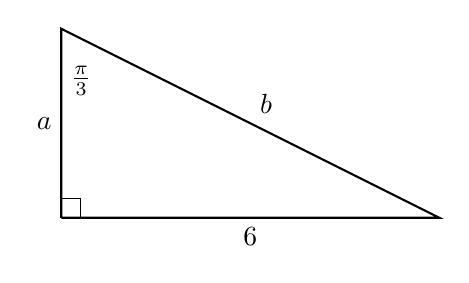
\begin{tikzpicture}[y=1.2cm, x=1.2cm,font=\sffamily]
        %% Draw the base, upright and hypotenuse
        \draw[thick] (0,0) -- (4,0) -- (0,2) -- (0,0); 
        \draw[thin] (0,0.1*2) -- (0.1*2,0.1*2) -- (0.1*2,0);
        \node[anchor=north] at (4/2,0) {$6$}; 
        \node[anchor=east] at (0,2/2) {$a$}; 
        \node[anchor=south west] at (4/2,2/2) {$b$};
        \node[anchor=south east,xshift=-24] at (4,0) {$$};
        \node[anchor=north west,yshift=-10] at (0,2) {$\frac{\pi}{3}$};
      \end{tikzpicture}
    \end{minipage}
    \begin{minipage}[h]{0.4\linewidth}
      \begin{eqnarray*}
        a & = & \\ [10pt]
        b & = & \\ [10pt]
      \end{eqnarray*}
    \end{minipage}

  \item ~ \\

    \begin{minipage}[h]{0.4\linewidth}
      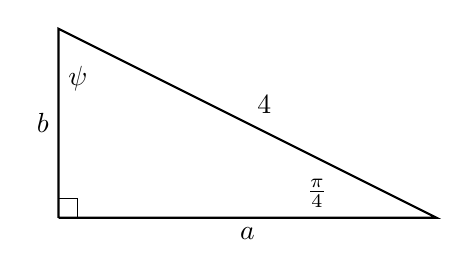
\begin{tikzpicture}[y=1.2cm, x=1.2cm,font=\sffamily]
        %% Draw the base, upright and hypotenuse
        \draw[thick] (0,0) -- (4,0) -- (0,2) -- (0,0); 
        \draw[thin] (0,0.1*2) -- (0.1*2,0.1*2) -- (0.1*2,0);
        \node[anchor=north] at (4/2,0) {$a$}; 
        \node[anchor=east] at (0,2/2) {$b$}; 
        \node[anchor=south west] at (4/2,2/2) {$4$};
        \node[anchor=south east,xshift=-36] at (4,0) {$\frac{\pi}{4}$};
        \node[anchor=north west,yshift=-10] at (0,2) {$\psi$};
      \end{tikzpicture}
    \end{minipage}
    \begin{minipage}[h]{0.4\linewidth}
      \begin{eqnarray*}
        a & = & \\ [10pt]
        b & = & \\ [10pt]
        \psi & = & \\ [10pt]
      \end{eqnarray*}
    \end{minipage}


    \item ~ \\

    \begin{minipage}[h]{0.4\linewidth}
      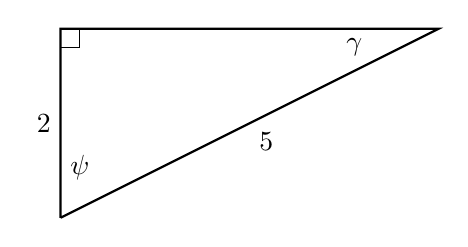
\begin{tikzpicture}[y=1.2cm, x=1.2cm,font=\sffamily]
        %% Draw the base, upright and hypotenuse
        \draw[thick] (0,0) -- (0,2) -- (4,2) -- (0,0); 
        \draw[thin] (0,0.9*2) -- (0.1*2,0.9*2) -- (0.1*2,2);
        %\node[anchor=south] at (4/2,2) {$a$}; 
        \node[anchor=east] at (0,2/2) {$2$}; 
        \node[anchor=north west] at (4/2,2/2) {$5$};
        \node[anchor=north east,xshift=-24] at (4,2) {$\gamma$};
        \node[anchor=south west,yshift=10] at (0,0) {$\psi$};
      \end{tikzpicture}
    \end{minipage} 
    \begin{minipage}[h]{0.4\linewidth}
      \begin{eqnarray*}
        \cos(\psi) & = & \\ [10pt]
        \sin(\psi) & = & \\ [10pt]
        \tan(\gamma) & = & \\ [10pt]
      \end{eqnarray*}
    \end{minipage}
    

  \end{enumerate}

\item If a 15 ft ladder is leaning against a wall at an angle of
  $62^\circ$ with the ground, how high up the will the ladder reach?
  Round to the nearest tenth of a foot.


\item Two observers are standing a distance of 100m apart. They both
  spot an eagle and watch it closely. The moment it passes between
  them, the first observer measures an angle of elevation from the
  ground of $45^\circ$ , and the second observer measures an angle of
  elevation from the ground of $35^\circ$ . How high in the air was
  the eagle when it passed between the two observers?

\item Prince Henry stands on the balcony of his castle that faces the
  sea. The base of the castle is 100m West of the beach, and the
  balcony is 30m above sea level. The Prince's true love, the commoner
  Matilda, is cleaning fish on a ship that is 200m directly East of
  the beach in a direct line East of the Prince's balcony. At that
  instant, as the Prince gazes upon his true love's ship, what is the
  angle of depression of his crying eyes?

\item Determine the exact value of $\sin(\omega)$.
  
    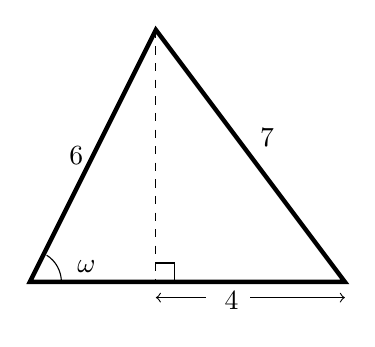
\begin{tikzpicture}[y=0.8cm, x=0.8cm,font=\sffamily]
      \draw[ultra thick,black] (0,0) -- (5,0) -- (2,4) -- cycle;
      \draw[black,dashed] (2,4) -- (2,0);
      \draw[black] (2,0.3) -- (2.3,0.3) -- (2.3,0);
      \node[anchor = south east] at (1.2,0)   {$\omega$};
      \node[anchor = east] at (1,2)         {$6$};
      \node[anchor = south west] at (3.5,2) {$7$};
      \node[anchor=north] at (3.2,0) {$4$};
      \draw[<-] (2,-0.25) -- (2.8,-0.25);
      \draw[->] (3.5,-0.25) -- (5,-0.25);
      \draw[black,thin] (0.5,0) arc (0:58:0.5);
    \end{tikzpicture}

\item Determine the exact value of $p$ in the figure below.

    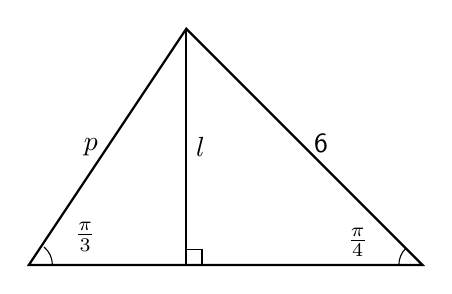
\begin{tikzpicture}[y=1.0cm, x=1.0cm,font=\sffamily]
      \draw[thick,black] (0,0) -- (2,3) -- (5,0) -- cycle;
      \draw[thick,black] (2,3) -- (2,0);
      \draw[thin,black] (2,0.2) -- (2.2,0.2) -- (2.2,0);
      \draw[thin,black] (4.7,0) arc (180:135:0.3);
      \draw[thin,black] (0.3,0) arc (0:50:0.3);
      \node[black,xshift=-23.4,yshift=8.2] at (5,0) {$\frac{\pi}{4}$};
      \node[black,xshift=20.4,yshift=10.2] at (0,0) {$\frac{\pi}{3}$};
      \node[black,anchor=south west] at (3.5,1.3) {6};
      \node[black,anchor=west] at (2,1.5) {$l$};
      \node[black,anchor=east] at (1,1.5) {$p$};
    \end{tikzpicture}


\item The area of a triangle is one half the length of its
  base multiplied by its height. Determine the area of the triangle
  shown below. \\ 
  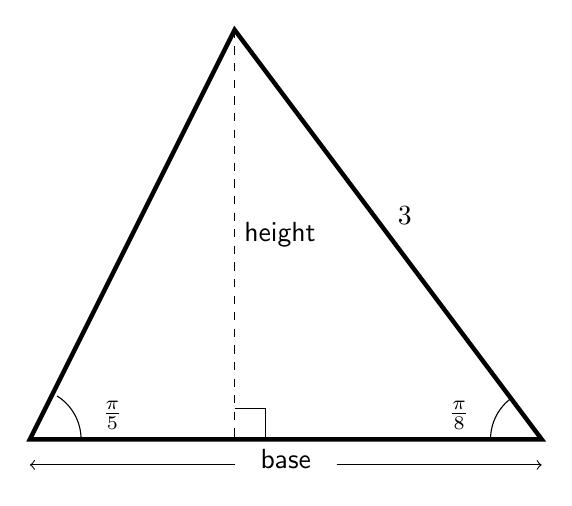
\begin{tikzpicture}[y=1.3cm, x=1.3cm,font=\sffamily]
    \draw[ultra thick,black] (0,0) -- (5,0) -- (2,4) -- cycle;
    \draw[black,dashed] (2,4) -- (2,0);
    \draw[black] (2,0.3) -- (2.3,0.3) -- (2.3,0);
    \node[anchor = south east] at (1.0,0)   {$\frac{\pi}{5}$};
    \node[anchor = south west] at (4.0,0)   {$\frac{\pi}{8}$};
    \node[anchor = south west] at (3.5,2) {$3$};
    \node[anchor = west] at (2,2) {height};
    \node[anchor=north] at (2.5,0) {base};
    \draw[<-] (0,-0.25) -- (2.,-0.25);
    \draw[->] (3,-0.25) -- (5,-0.25);
    \draw[black,thin] (0.5,0) arc (0:58:0.5);
    \draw[black,thin] (4.5,0) arc (180:125:0.5);
  \end{tikzpicture}

\item A person is standing forty meters from the base of a building,
  and the person is looking directly at a point halfway to the top of
  the building. The angle of elevation is $32^\circ$.  What will the
  angle of elevation be when the person is looking at the top of the
  building?

\item Sir Edmund Hillary is standing between two peaks, Mount Dampier
  and Mount Vancouver.  It is estimated that the two peaks are the
  same height. Sir Hillary is standing in a line directly between the
  two peaks, and he estimates that his distance to a point directly
  below the peak of Mount Dampier at his same altitude is seven
  hundred meters more than the distance to the equivalent point below
  Mount Vancouver. When looking at Mount Dampier he estimates the
  angle of elevation is $41.6^\circ$, and his angle of elevation for
  Mount Vancouver is $69.4^\circ$. What is the elevation of the two
  peaks above Sir Hillary's current elevation?

\end{enumerate}



  
